\subsection{Umsetzung der GUI im Code}\label{tkintercode}
\paragraph{Klassenstruktur}
Im Vordergrund basiert die Klassenstruktur grundsätzlich auf \gls{gls_ctk} Komponenten (siehe Abb.~\ref{fig:klassenstruktur_frontend}). Dabei gibt es die Klassen \enquote{App}, \enquote{PageFrame}, \enquote{TitleFrame} und \enquote{MeasurementFrame}. Im Programm wird eine \enquote{App} Instanz ausgeführt, welche das Hauptfenster ist. Diese Instanz kann beliebig viele \enquote{PageFrames} enthalten, die wiederum jeweils ein \enquote{TitleFrame} und eine Liste von \enquote{MeasurementFrames} beinhalten. Die \enquote{PageFrames} stellen die einzelnen Seiten dar, welche per Knopfdruck an der \acs{rltanzeige} durchgeblättert werden können. In einem \enquote{TitleFrame} wird immer der Titel der jeweiligen Seite gespeichert \bzw angezeigt. In den \enquote{MeasurementFrame} Instanzen werden hingegen die tatsächlichen Messwerte (Bezeichnung + Wert + Maßeinheit) dargestellt.

\begin{figure}[H]
	\centering
	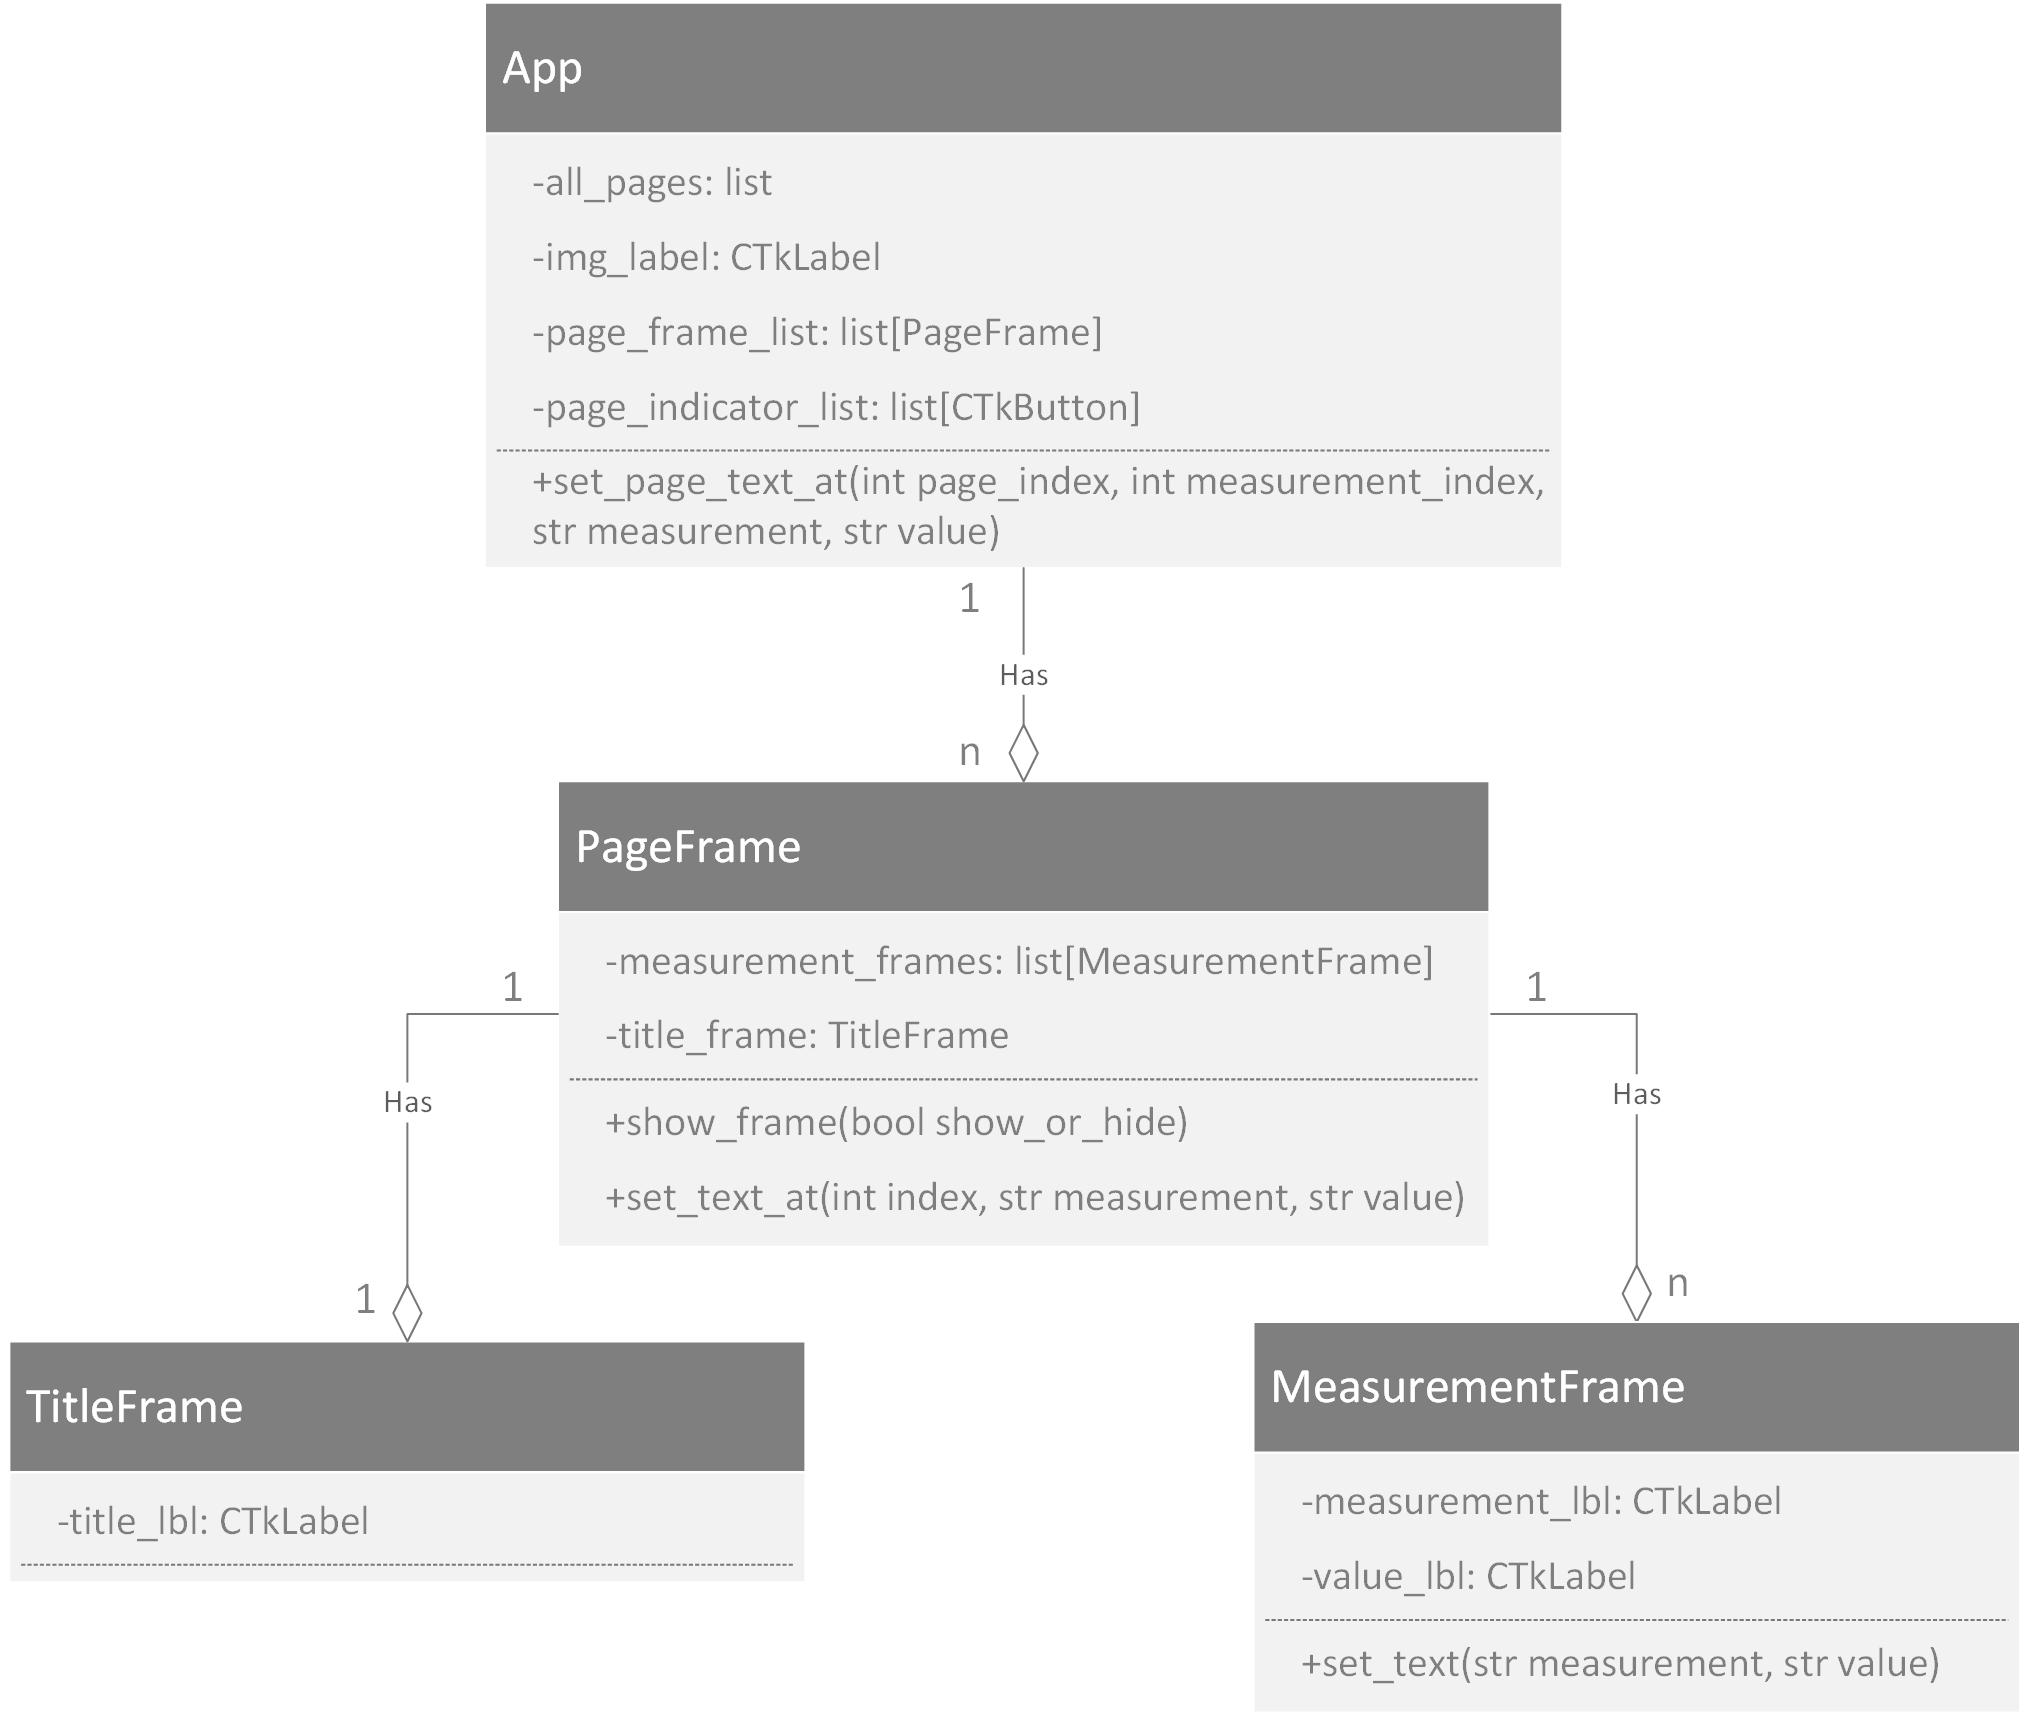
\includegraphics[width=0.95\textwidth]{uml_frontent_class_diagram}
	\caption{UML Diagramm Frontend \label{fig:klassenstruktur_frontend}}
\end{figure}

\paragraph{CustomTkinter Code}
Eine nähere Beschreibung und die Umsetzung der vorher genannten Klassen erfolgt in diesem Kapitel. 
\newline Wie zuletzt beschrieben, basieren alle Klassen im Frontend auf \gls{gls_ctk}. Die Klassen sind dabei alle (bis auf die Klasse \enquote{App}) vom Typ \enquote{CTkFrame}. Ein \enquote{CTkFrame} ist ein Widget, das wie ein Rahmen \bzw Behälter für andere Widgets fungiert. So können diese in weiteren Widgets gruppiert und besser organisiert werden. Als erster Parameter wird für \enquote{CTkFrames}, wie bei allen \gls{gls_tk} und \gls{gls_ctk} Widgets, der \enquote{master} \bzw das Elternobjekt angegeben. Darüber hinaus können die Breite (\enquote{width}), Höhe (\enquote{height}), Rahmenbreite \bzw -Farbe (\enquote{border\_width} \bzw \enquote{border\_color}) sowie die Hintergrundfarbe (\enquote{fg\_color}) angegeben werden. \cite[vgl.][]{Schimansky:o.J.}

Die Klasse \enquote{TitleFrame} enthält ein \enquote{CTkLabel}, welches mit der \enquote{place( )} Methode im Behälter platziert wird. Die Klasse \enquote{CTkLabel} basiert auf der Klasse \enquote{tkinter.Label} und dient zur Darstellung eines Textes. Im \enquote{TitleFrame} Label steht immer der Titel der zugehörigen Seite. Das \enquote{title\_font} Objekt, welches im folgenden Code zu sehen ist, ist eine Instanz der \gls{gls_ctk} Utility Klasse \enquote{CTkFont}. Es wird verwendet, um die Schriftformatierung von \gls{gls_ctk} Widgets vorzunehmen. Jedes \gls{gls_ctk} Widget bekommt standardmäßig ein \enquote{CTkFont} Objekt, wobei ein solches Objekt zeitgleich mehreren Widgets angefügt werden kann. Eine Änderung eines \enquote{CTkFont} Objekts wird an alle Widgets, die es verwenden, weitergeleitet. \cite[vgl.][]{Schimansky:o.J.}

\begin{pythoncode}
class TitleFrame(ctk.CTkFrame):
	def __init__(self, master, title, **kwargs):
		super().__init__(master, width=800, height=60, fg_color=text_color, **kwargs)
		
		title_font = ctk.CTkFont(family="Roboto", size=32)
		
		self.title_lbl = ctk.CTkLabel(master=self, text=title, width=700, height=45, fg_color="transparent", text_color=title_color, anchor=ctk.CENTER, font=title_font)
		self.title_lbl.place(relx=0.5, rely=0.12, anchor=ctk.N)
\end{pythoncode}

Wie in der Klassenstruktur beschrieben, beinhaltet ein jedes \enquote{PageFrame} neben einem \enquote{TitleFrame} eine Liste von \enquote{MeasurementFrames}. Eine Instanz der Klasse \enquote{MeasurementFrame} enthält immer Informationen zu einem bestimmten Messwert, welche mithilfe von zwei \enquote{CTkLabel} Widgets dargestellt werden. Dabei wird die Bezeichnung des Messwerts links im \enquote{measurement\_lbl} und der tätsichliche Wert einschließlich Maßeinheit rechts im \enquote{value\_lbl} platziert. Die zwei Labels werden durch einen Strich getrennt, der mit dem \gls{gls_tk} Widget \enquote{Canvas} erstellt wird. Ein Canvas ist ein rechteckiger Bereich \bzw eine Leinwand, auf dem Bilder oder andere komplexe Layouts gezeichnet werden können. Zusätzlich lassen sich auf einem Canvas Widget \zB weitere Widgets, Text oder Bilder platzieren. \cite[vgl.][20]{Shipman:2013} 
\newline Da jeder Messwert kontinuierlich aktualisiert wird, verfügt die \enquote{MeasurementFrame} Klasse über die Methode \enquote{set\_text}. In dieser wird mithilfe der \enquote{configure( )} Methode der Text beider Labels aktualisiert. Es folgt ein gekürzter Code zur \enquote{MeasurementFrame} Klasse.

\begin{pythoncode}
class MeasurementFrame(ctk.CTkFrame):
	def __init__(self, master, measurement, value, **kwargs):
		#[Initialisierung des CTkFrames + Erstellung eines CTkFont Objekts zur Schriftformatierung der MeasurementFrames]
		
		self.measurement_lbl = ctk.CTkLabel(master=self, text=measurement, ...)
		self.value_lbl = ctk.CTkLabel(master=self, text=value, ...)
		self.canvas = Canvas(master=self, ...)
		#[Platzierung beider Labels + Canvas]
		
	def set_text(self, value):
		self.value_lbl.configure(text=value)
\end{pythoncode}

Die letzte der \gls{gls_ctk} \enquote{CTkFrame} Klassen ist die \enquote{PageFrame} Klasse. Wie bereits erwähnt ist jede Instanz dieser Klasse ein unsichtbarer Behälter, der ein \enquote{TitleFrame} sowie eine Liste von \enquote{MeasurementFrames} beinhält und als Seite dient. Diese Komponenten werden, wie im nachstehenden Code zu sehen ist, im Konstruktor eines jeden \enquote{PageFrames} zugeordnet. Die Parameter \enquote{title} und \enquote{measurement} stammen aus der \acs{json} Haupt-Konfigurationsdatei (siehe Kapitel \ref{json_config_files}, Tab. \ref{tab:pages_array_parameter} unter \enquote{title} \bzw Tab. \ref{tab:sources_array_parameter}  unter \enquote{description}) und können daher schon bei Erstellung der \enquote{PageFrame} Instanzen übergeben werden. Der \enquote{value} Parameter der individuellen \enquote{MeasurementFrames} hingegen wird laufend von der Methode \enquote{set\_text\_at( )} aktualisiert und ist daher am Anfang bis zum ersten Auslesen auf \enquote{N/A} (\dt nicht verfügbar) gesetzt.
	
\begin{pythoncode}
class PageFrame(ctk.CTkFrame):
	def __init__(self, master, title, parameters, **kwargs):
		#[Initialisierung des CTkFrames]
		self.measurement_frames = []
		self.title_frame = TitleFrame(master=master, title=title, ...)
		
		for parameter in parameters:
			frame = MeasurementFrame(master=master, measurement=parameter.description, value="N/A", ...)
			self.measurement_frames.append(frame)

    def set_text_at(self, index, value):
        self.measurement_frames[index].set_text(value)
...
\end{pythoncode}

Die \enquote{PageFrame} Klasse enthält zudem eine \enquote{show\_frame( )} Methode, die dazu dient die jeweilige \enquote{PageFrame} Instanz \bzw ihren Inhalt sichtbar oder unsichtbar zu machen. Diese Methode ist notwendig, um zwischen den unterschiedlichen Seiten wechseln zu können \bzw die Seitenstruktur (siehe Kapitel \ref{figma_design}) für die jeweilige \acs{rltanzeige} umzusetzen.

\begin{pythoncode}
...
	def show_frame(self, show_or_hide):
		if show_or_hide:
			self.title_frame.place(...)
			self.title_frame.tkraise()
		else:
			self.title_frame.place_forget()
		
		for my_frame in self.measurement_frames:
			if show_or_hide:
				my_frame.place(...)
				my_frame.tkraise()
			else:
				my_frame.place_forget()
\end{pythoncode}

Die Klasse \enquote{App} ist eine Instanz der \gls{gls_ctk} Window Klasse \enquote{CTk}. Die \enquote{CTk} Klasse bildet als Hauptfenster die Grundlage für jedes \gls{gls_ctk} Programm. Dabei sollte während der Laufzeit eines Programmes immer nur eine Instanz der \enquote{CTk} Klasse existieren, wobei weitere Fenster mit der \enquote{CTkToplevel} Klasse erstellt werden können. Mit Aufruf der \enquote{mainloop( )} Methode wird das Programm gestartet.
\cite[vgl.][]{Schimansky:o.J.} 

Folgend ist ein vereinfachter Code des Konstruktors der Klasse \enquote{App} zu sehen. Hier wird das Hauptfenster aufgesetzt. Dabei wird zuerst mit den Methoden \enquote{attributes( )}, \enquote{resizable( )} und \enquote{config( )} die Größe des Fensters festgelegt, sowie der Cursor deaktiviert, da die \acs{rltanzeige} durch Knöpfe gesteuert wird und dieser daher irrelevant ist. Daraufhin wird das Logo der Firma Bösch hinzugefügt. Dafür kommt die \gls{gls_ctk} Utility Klasse \enquote{CTkImage} zum Einsatz, die als Behälter für das Bild dient und wiederum mithilfe eines \enquote{CTkLabels} im Hauptfenster platziert wird.

\begin{pythoncode}
class App(ctk.CTk):
	def __init__(self, all_pages, page_frame_list, page_indicator_list, *args, **kwargs):
		super().__init__(*args, **kwargs)
		self.attributes('-fullscreen', True)
		self.resizable(False, False)
		self.config(cursor="none")
		
		boesch_logo = ctk.CTkImage(light_image=Image.open("..."), dark_image=Image.open("..."), size=(x, y))
		self.img_label = ctk.CTkLabel(master=self, image=boesch_logo, text="")
		self.img_label.place(...)
...
\end{pythoncode}

% Weiters werden im Konstruktor die globalen Listen \enquote{page\_frame\_list } und \enquote{page\_indicator\_list} erstellt, die zur Verwaltung der \enquote{PageFrames} sowie Indikatoren für die Seitenanzeige dienen.

Weiters wird im Konstruktor für jede \enquote{Page} in der Liste \enquote{all\_pages} ein \enquote{PageFrame} erstellt und der \enquote{page\_frame\_list} hinzugefügt. Die Liste \enquote{all\_pages} ist eine Liste mit allen nötigen Informationen für ein \enquote{PageFrame} und wird im Backend des Programmes erstellt (siehe Kapitel \ref{auslesen_rlt_parameter}). Die \enquote{page\_frame\_list} ist eine globale Liste, die zur Verwaltung der \enquote{PageFrames} dient. Anschließend wird das erste \enquote{PageFrame} sichtbar gemacht, indem die Methode \enquote{show\_frame(True)} aufgerufen wird.

\textbf{\textit{VISIO VERÄNDERN!!! GLOBALE LISTEN/VARIABLEN AUS DER APP KLASSE ENTFERNEN!}}

\begin{pythoncode}
...	
		for page in all_pages:
			page_frame_list.append(PageFrame(master=self, title=page.title, parameters=page.measurements))
   
		page_frame_list[0].show_frame(True)
...
\end{pythoncode}

Zuletzt werden im Konstruktor die Seitenindikatoren erstellt und platziert. Jeder Indikator wird mithilfe des \gls{gls_ctk} Widgets \enquote{CTkButton} erstellt und ist somit grundsätzlich ein grauer, runder Knopf ohne Text. Eine besonderheit ist dabei, dass der Knopf mithilfe der globalen Variable \enquote{current\_page} erkennen kann, ob er Hellgrau oder Dunkelgrau wird, wenn seine zugehörige Seite angezeigt wird.

Die Position der Seitenindikatoren wird basierend auf der Anzahl der Seiten dynamisch berechnet. Wenn mehr als eine Seite vorhanden ist, wird für jede Seite in der Liste \enquote{page\_frame\_list} ein Indikator erstellt und platziert, wie im folgenden Code vereinfacht gezeigt wird.

\begin{pythoncode}
...
		if len(page_frame_list) > 1:
			for i in range(0, len(page_frame_list)):
				page_indicator_list.append(ctk.CTkButton(master=self, ..., fg_color=("hellgrau" if i == current_page else "dunkelgrau")))
				page_indicator_list[i].place(relx=start_x_position + number,...)
...
\end{pythoncode}

Die Klasse \enquote{App} beinhaltet eine Methode mit dem Namen \enquote{set\_page\_text\_at( )}. Sie wird in der \enquote{data\_refresh( )} Methode aufgerufen (siehe Kapitel \ref{auslesen_rlt_parameter}), welche dazu dient, die Messwerte regelmäßig zu aktualisieren.

\begin{pythoncode}
	def set_page_text_at(self, page_index, measurement_index, value):
    	page_frame_list[page_index].set_text_at(measurement_index, value)
\end{pythoncode}
